\documentclass[a4paper, 12pt]{article}

%better bibliography style control
\usepackage{natbib}

%utf-8, because it is the default in linux these days
\usepackage[utf8]{inputenc}

%\usepackage{graphicx}
\usepackage[pdftex]{color,graphicx}
\usepackage{hyperref}

%make the url links blue
\hypersetup{
    pdfauthor={Eduardo Bellani},
    pdftitle={An emergent participatory design framework for higher education},
    pdfkeywords={education, emergent design, culture, technology},
    colorlinks,
    urlcolor= blue
}


\title{An emergent participatory design framework for higher education}

\author{Eduardo Bellani}

\begin{document} 
    \maketitle
    \begin{abstract}
    Our current society is exponentially increasing its dependency on technology
    and science, and this dependence is likely to get deeper in the close
    future. The current educational system is broken even for the needs of past
    decades, and it is a bad joke to consider it satisfactory for our current
    and future needs. This leads to a dangerous situation where a society will
    have a base that very few of its members comprehend.

    The educational proposal that I outline here leverages current technologies
    to create the condition where people can have access to top notch knowledge
    and technologies, so that a more democratic and efficient pedagogical
    approach can emerge, one that is more encompassing and that allows for much
    more personal control over the process.
    \\
    \\
    \textbf{keywords}: education, technology, constructionism, emergent
\end{abstract}


    \section{Introduction}


Two fundamental concepts form the basis of the educational system this article is trying to
communicate. One is constructionism, a theory developed by Seymour Papert, and
it is the epistemological approach that runs throughout the system, and affects
how the learning (and consequently the teaching) process is viewed. The second
one is emergent design, and that is the organizational and structural view of
the system, and affects how the system evolves and relates to its members and
environment. Both concepts are intertwined, as will be shown below. 

\subsection{Constructionism}
Constructionism is an epistemological theory that was developed by Seymour
Papert, drawing from his experiences as a mathematician, his time studying with
Jean Piaget (the developer of the constructivist theory) in France and from his
background as an artificial intelligence and media researcher.

\cite{education:cavallo_building_knowledge} makes a clear distinction between Constructionism and
Constructivism:

\begin{quote}
  Constructionism builds upon principles in constructivism. While constructivism
  holds that the learner constructs new knowledge based on the existing knowledge
  he or she has, constructionism builds on this idea by maintaining that this
  process happens particularly well when the learner is in the process of
  constructing something.                   
  
\end{quote}

Constructionism is also a true pedagogy of autonomy, in a very Freirean way:
\begin{quote}
...teaching is not transferring knowledge, but creating opportunities for their own
production or its construction.
\cite{education:paulo_freire__pedagogia_da_autonomia}
\end{quote}

We can observe the deep connection of constructionism with computers and
technology. But that is far from a technocentrist, where technology is used just
for the sake of using technology. That connection comes from the almost endless
capacity of the computer to create simulations and concept of microworlds:

\begin{quotation}
Learners in a physics microworld are able to invent their own personal sets of
assumptions about the microworld and its laws and are able to make them come
true.  They can shape the reality in which they will work for the day, they can
modify it and build alternatives.  This is an effective way to learn,
paralleling the way in which each of us once did some of our most effective
learning. Piaget has demonstrated that children learn fundamental mathematical
ideas by first building their own, very much different (for example,
preconservationist) mathematics. And children learn language by first learning
their own ("baby-talk") dialects. So, when we think of microworlds as incubators
for powerful ideas, we are trying to draw upon this effective strategy: We allow
learners to learn the "official" physics by allowing them the freedom to invent
many that will work in as many invented worlds.
\cite{education:papert_mindstorms}
\end{quotation}

That kind of characteristic is crucial to deeper changes in education and what
is meant by knowing. 

\begin{quotation}
The need to distinguish between a first impact on education and a deeper meaning
is as real in the case of computation as in the case of feminism. For example,
one is looking at a clear case of first impact when "computer literacy" is
conceptualized as adding new content material to a traditional curriculum.
Computer-aided instruction may seem to refer to method rather than content, but
what counts as a change in method depends on what one sees as the essential
features of the existing methods. From my perspective, CAI amplifies the rote
and authoritarian character that many critics see as manifestations of what is
most characteristic of--and most wrong with--traditional school. Computer
literacy and CAI, or indeed the use of word-processors, could conceivably set up
waves that will change school, but in themselves they constitute very local
innovations--fairly described as placing computers in a possibly improved but
essentially unchanged school. The presence of computers begins to go beyond
first impact when it alters the nature of the learning process; for example, if
it shifts the balance between transfer of knowledge to students (whether via
book, teacher, or tutorial program is essentially irrelevant) and the production
of knowledge by students. It will have really gone beyond it if computers play a
part in mediating a change in the criteria that govern what \emph{kinds of knowledge
are valued in education.} 
\cite{education:papert__situating_constructionism}
\end{quotation}


\subsection{Emergent Design}

Emergent design is a strategy for building systems that are too complex to be
tackled in a top down, plan first manner, as
\cite{education:cavallo__technological_fluency} puts is:
\begin{quotation}
Popular views about design, about reform, about planning, about control
typically lag behind progress. New organizations are pioneering new means of
control and change.  Emergent design is the recognition that certain systems are
too complex, dynamic, interconnected, and chaotic to attempt to manage them by
top-down, pre-planned, rigid means of control. Large educational systems are
one-such system. The human brain is another.  That this project is
simultaneously involved with both systems is all the more reason to take an
emergent approach.
\end{quotation}

So the point of the strategy is to build systems that provide a base for systems
to be built on it, by the users of the system itself. A global participatory architecture
that connects several systems that grew on top of it. That view has several
advantages as \cite{education:cavallo__technological_fluency} objectives for workshops in his emergent design system in
Thailand shows:

\begin{quote}
  The workshops were intended to:
  \begin{itemize}

 \item provide powerful personal
experiences of a different approach to learning,

 \item break pessimistic mindsets about people’s ability to learn,

 \item surface, reflect upon and discuss participants’ own prior explicit and
 implicit assumptions about learning to the surface, and compare them to the new
 experience,

 \item encourage participants to think about the learning process itself,

 \item engage in thinking about the design and practice of learning environments
 in the local context,

 \item identify local people whose thinking and acting appear promising so that
 they can take on greater roles for change,

 \item debug our own thinking about the mechanisms of learning and our own
 pattern of practice in designing learning environments.  

 \end{itemize}
\end{quote}

\subsection{Why}

But why propose of a new system for higher education, one that puts the learner
in the driver seat, that can growth organically with a community and is deeply
connected to what is important for an individual and his community? Because I see that the act of
descholling society, in the sense of individuals empowering themselves, is
critical for the current and future society that wishes to remain democratic.

\cite{education:cavallo__models_of_growth} quotes John Dewey on exactly this fact:
\begin{quote}
For Dewey a just society could only be built not based upon the dictates of
clergy, royalty, or an elite, but depended upon the informed collective
decisions of all, where every voice should be heard.
\end{quote}

But what descholling means, and to who falls the responsibility for deschooling
an individual? \cite{education:ivan_illich__deschooling_society} provides a
clear answer to both questions.

\begin{quotation}
  Only liberating oneself from school will dispel such illusions. The discovery
  that most learning requires no teaching can be neither manipulated nor planned.
  Each of us is personally responsible for his or her own deschooling, and only we
  have the power to do it. No one can be excused if he fails to liberate himself
  from schooling. People could not free themselves from the Crown until at least
  some of them had freed themselves from the established Church. They cannot free
  themselves from progressive consumption until they free themselves from
  obligatory school.
\end{quotation}

So if we analyze that the current and next generations of children, poor and rich alike, are
growing along with computers and their powerful integration capabilities, and
the aim of projects like the OLPC is: 

\begin{quote}
    to adequately educate all the children of the
    emerging world. Simply doing more of the same is no longer enough, if it
    ever was. If their citizens are to benefit, as they should from the spread
    of the technology-based, global information economy, these nations must
    rethink the old top-down classroom paradigm. 
    \cite{education:olpc_educational_proposition}
\end{quote}

What can we say about the next educational step for those children, higher
education, in this context?
Certainly a person who grew used to those conditions in their development 
would find the current state of affairs in university appalling. 

\cite{futurism:kurzweil_singularity_is_near}, in his book tries to make a point
about the importance of the exponential pace of technological development, and
how it will affect the individual and the society as a whole on all conceivable
aspects on a very close future.  A society that does not prepare it's citizens
for such future is doomed to become mere spectator and follower of those who do.
A small account of his view of the present educational situation perhaps
illustrates the point better:

\begin{quotation}
    Most education in the world today, including in the wealthier communities,
    is not much changed from the model offered by the monastic schools of
    fourteenth-century Europe. Schools remain highly centralized institutions
    built upon the scarce resources of buildings and teachers. The quality of
    education also varies enormously, depending on the wealth of the local
    community (the American tradition of funding education from property taxes
    clearly exacerbates this inequality), thus contributing to the have/have not
    divide.
\end{quotation}

The impact of delaying, however, is not only social, but profoundly individual as well, as
\cite{education:papert_gaston_vision_for_education} puts it, ``So the choice is
not whether we will consider deep changes in school but how many children will
be lost before we recognize that we have to do so'', or in other words on the
same work:
\begin{quotation}
    As the slow evolution of school lags further and further behind the rapid
    evolution of society, increasing numbers of students all over the world see
    school as irrelevant to life. Many drop out. Many more drop out mentally,
    emerging from school with poor skills and negative visions of themselves and the
    society they are entering.
\end{quotation}

    \section{Description}

The overall system has the objective of graduating individuals in a manner that
is at the same time democratic, stimulating, meritocratic and able to prepare 
those same individuals for a life in a society where computers will
play a major role.

In order to do that with a decreased cost, both financial and social, it is wise
to use the existing structure where it is possible to do so, so that factor is
embedded in the project as well.

\subsection{The relationship with knowledge}

The first step of the system would be the self preparation of a given student
through a process of interaction with the knowledge. But what knowledge? Well,
before the system is constructed it will be the job of the competent
authorities, both private and public, to digitalize the best available content
of the existing superior educational system. That could be done through the
video capturing of the federal universities classes, plus the digitalization of
all the non copyrighted material. 

That content should be placed in a free and open environment in the internet,
where it would be available to every citizen that would be interested in it.
This system would be described only superficially here, because ideally it would
leverage all the modern existing web development techniques in the ``web 2.0''.
Those techniques would serve to guide the students, to promote socialization in
the form of forums, tests, iterative games and so on, where the students would
play not only with the resources available on the system, but with each other
projects and exercises. That, as Papert puts it, places the fun on the learning
process:

\begin{quotation} 
    Part of the fun is sharing, posting graphics on the walls, modifying and
    experimenting with each other's work, and bringing the ``new'' products back to
    the original inventors. Although the work at the computer is usually private it
    increases the children's desire for interaction. These children want to get
    together with others engaged in similar activities because they have a lot to
    talk about. 
    \cite{education:papert_mindstorms}
\end{quotation}

This space would, of course, grow in richness with every user increasing the
opportunities and sharing it's own epistemological experiences, not only in some
particular subjects, which of course would take place, but of the medium itself,
smoothing the learning curve with each generation of users and producing a more
fitted social intelligence in the process, like Papert again makes clear:

\begin{quotation}
    As with writing, so with music-making, games of skill, complex graphics,
    whatever: The computer is not a culture unto itself but it can serve to
    advance very different cultural and philosophical outlooks.
    \cite{education:papert_mindstorms}
\end{quotation}

Of course, one does not expect the users would be the only responsibles for the
system. The hired professors of the competent authorities should be available
with enough consistency to increase the quality of the discussions and of the
official content of the system. 

One important aspect is that the form of the courses could be highly flexible,
which means that one could approach some subject from several points of view,
according to one's own pace and vocation. That would be a form of Piagetian
thinking, because although there would be goals, as the it will be discussed
later, the student is completely free to choose how and when to face those goals,
and if they would be faced at all. 

\subsection{The guarantee of quality}

A skeptical of the last scenario could, with quite a lot of reason, ask: ``But
what about the quality of those students, or should we just hand diplomas to
everyone who claims to be ready?''. Our society clearly must have a way to
assure itself of the quality of those who want to perform critical functions,
such as engineers, physicians and several other professions who deal with human
life in their craft.    

The way that was proposed so far concerned itself with the student acquiring and
holding the knowledge. But what about testing? To that we should turn to what
society usually turns to find credibility, specialized institutions and the
government, and those credible institutions could build a streamlined, on-demand 
certification scheme. More specifically in the Brazilian case, the very
structure of the vestibular system (which is highly effective and encompassing)
could be used to certificate students on general or specific points. Those
authorities would have control over the tests and what set of tests would
encompass a given course. 

For instance, to be fully graduated in medicine one should have to complete the
certifications of medicine 1 all the way through medicine 10, each sequentially
and with a minimum grade. To ask for a given test to be applied some person
would only have to provide some documentation and pay some fee to cover the
costs of using the system, and in the next round of testing the wanted test
would be available on some testing facility that is nearest to the requirer. The
testing procedure per se would be audited by payed officers. The system would
indeed be the same as a normal vestibular.


\subsection{The needed physical step}

The model so far would be incomplete on our day and age, mostly because of the
limitations of the digital distribution model. That will probably change if we
follow Kurzweil ideas:

\begin{quotation}
    Because of current bandwidth limitations and the lack of effective
    three-dimensional displays, the virtual environment provided today through
    routine Web access does not yet fully compete with ``being there'', but that
    will change. In the early part of the second decade of this century
    visual-auditory virtual- reality environments will be full immersion, very
    high resolution, and very convincing. Most colleges will follow MIT's lead,
    and students will increasingly attend classes virtually. Virtual
    environments will provide high-quality virtual laboratories where
    experiments can be conducted in chemistry, nuclear physics, or any other
    scientific field. Students will be able to interact with a virtual Thomas
    Jefferson or Thomas Edison or even to \textit{become} a virtual Thomas
    Jefferson. Classes will be available for all grade levels in many languages.
    The devices needed to enter these high-quality, high-resolution virtual
    classrooms will be ubiquitous and affordable even in third world countries.
    Students at any age, from toddlers to adults, will be able to access the
    best education in the world at any time and from any place.
    \cite{futurism:kurzweil_singularity_is_near} 
\end{quotation}

But what could be done today to reproduce the physical training and
socialization required for the formation of a fully fledged professional or
researcher? That today would still need a physical gathering place. 

The steps explained earlier would provide that space, by freeing up the existing
classrooms that before were dedicated to teaching repeatedly stuff. Not only the
classrooms would be liberated, but the professors would be alleviated of most of
the burden of direct teaching the horde of new students that would arrive each
semester.   

If both professors and classrooms would have more capability, so workshops could
be created based on demand, and labs could use students with some
qualifications or characteristics for assistants. There would be a very lively
interplay between the institutions and those who wanted to partake on those
activities, and that process would be guided much by the individual, choosing
when and how to approach the institution. 

Those labs and workshops could, if certified by the authorities, also certify
students who are active on them, so there would be an extra motivation for
students to build their own projects, in a very constructionist way.

\clearpage

\subsection{Overview}

\begin{figure}[htb]
   \centering
   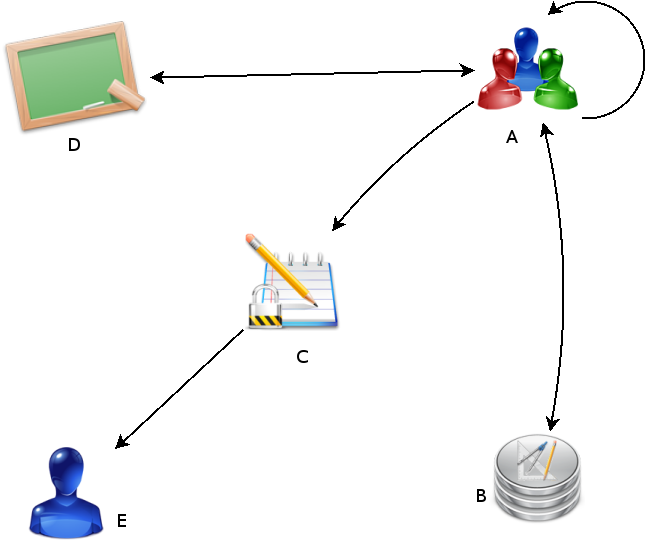
\includegraphics[width=1\columnwidth]{images/diagram.png}
   \caption{Overview diagram}
   \label{fig:overview_diagram}
\end{figure}


\begin{description}
    \item[A] The population interested in the system, the candidates.
    \item[B] The knowledge made available by the institutions.
    \item[C] The certification procedure.
    \item[D] The labs with a physical location, operated by faculty, mentors and the
    certificated students.
    \item[E] A graduated student.
\end{description}


    \section{An hypothetical case}


Hi. My name is John Doe, and I've just graduated from high school. I'm a bit
undecided about what to do now, what path to follow. My mom  says that an
attorney is a really respected profession, and I could earn a lot of money so I
could help her afterwards, so I'll take a shot a Law.

I'm a poor person, so I don't have any money to afford a private university. And
the public ones are so competitive that I would have to stop working and focus
for a long time on studying for the vestibular just to have a shot to be
admitted. But I've heard of a new program by the federal government that
eliminates the need for a vestibular, and gives me the liberty of studying at my
own pace and time, but it uses computers and my family doesn't have one, by the
obvious reason of having to buy food instead.

But there's a new computer center that the government opened at my community,
and they say one of their objectives is to attend to people in situations like
mine, so I'll schedule appointments on there.

\textit{six months later \ldots }

I'm studying every day for the second certification. In the first four months
I've learned enough to pass the first one with a acceptable grade. I'm planning
to study more this time to make it with a higher grade. People say that
university has plenty of vacancy without all this subjects on the classroom, but
I don't know how it will be when I finish all the certifications, so it's better
to be safe than sorry.

The materials are fun, and I've met several people who were studying the same
subjects, and we kind of help each other on the suggested lessons and
assignments. I think the next test will be hard, but with each passing day I'm
learning more to communicate my questions on-line and I think I'll make it
through.

\textit{a couple of years later \ldots }

I've made it! I've went through all the necessary certifications with a
satisfactory enough grade, and now I have been called into a model forum on a
federal facility for students! I feel ready for it, although a bit nervous, 
but at least this forum is on my town, and perhaps I could help my own community
through my work and knowledge.

\textit{a year and a half later \ldots }

I'm almost finished with my work at the forum. I've met several students and
professors, but the most pleasurable experience was to help families similar to
mine on the process. 

I've applied my knowledge directly on the field, and frankly, my certifications
did come in handy, because I had a intellectual security to handle a lot of
different situations, and the ones I didn't knew how to handle I used the same
research process I've used back on my home study days to figure it out. In some
months my graduation will take place, I'll miss this my colleagues, but I'm also
anxious to get on the market and flourish as a professional...




    %    Thus, conclusions should be short and sweet. Do not restate all of your findings. One
%statement in the abstract, one in the introduction and once more in the body of the text
%should be enough! You can include a short paragraph or two acknowledging limitations,
%suggesting implications beyond those in the paper. Keep it short though — don’t write your
%grant application here outlining all of your plans for future research. And don’t speculate;
%the reader wants to know your facts not your opinions.

%Conclusion
%
%To summarize, I am presenting for computer science an argument that has come up before in many other areas of science and mathematics education. Our official curricula, I think, run the same risk as the official physics curriculum that caused Albert Einstein to drop out of school. Such rigidity would be particularly regrettable in a subject like computer programming, which lends itself so readily to a flexible, experimental approach. 
%
%

\section{Conclusion}

Summarizing, I am presenting an argument for an emergent design approach for
education systems, one that is based on an approach for emergent design detailed
by \cite{education:cavallo__technological_fluency} and that uses as its
pedagogical and epistemological base constructionism, as situated in
\cite{education:papert__situating_constructionism}.

This article ends with the words of
\cite{education:resnick&ocko_learning_through_design} that I find very relevant
for systems like the one I proposed so far:

\begin{quote} 
    Implementing these strategies is not easy. There are many unanswered
    questions--such as how to help students ``break away'' from their initial
    ``regions of comfort.'' And coordinating open-ended design activities is a
    challenge for any teacher. Indeed, organizing an ``Inventor's Workshop'' is
    far more difficult than delivering a lecture on mechanical advantage, or
    developing a step-by-step hands-on lesson. As
    \cite{education:dewey_experience_education} noted more than a half-century
    ago (in words that still ring true today): ``The road of the new education
    is not an easier one to follow than the old road but a more strenuous and
    difficult one.'' But it is a road well worth taking. 
\end{quote}



    \bibliographystyle{plainnat}
    \bibliography{references}
\end{document}
